\begin{figure}
\chapter{Development Timeline}
The Development Timeline is a graphical representation of all the tasks that are needed for the completion of the project. This graphical model is known as Gantt Chart.
\newline
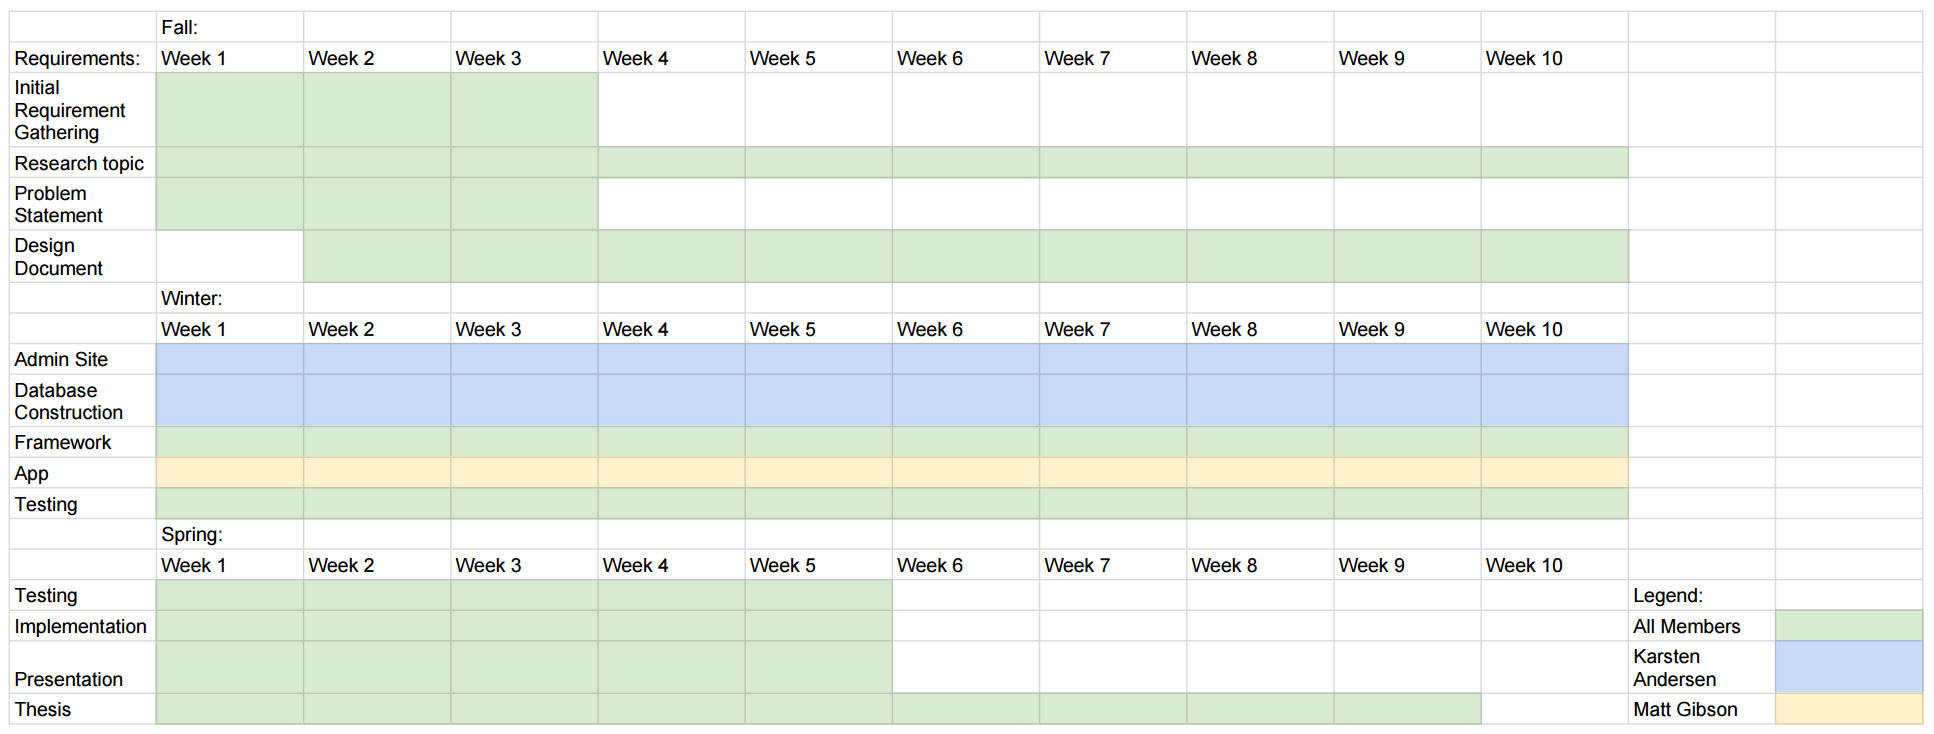
\includegraphics[width=1\textwidth]{images/gantt.png}
\caption{Gantt Chart}
The table columns in the Gantt Chart lists the set time periods over which the project is distributed in. For our purpose, we have divided the project across ten weeks for each quarter. The rows of the table in the chart lists the various tasks that need to completed. The intersection of the rows and columns in the Gantt Chart would provide data about the team member who will be working on a respective task and when a particular task is due for submission or presentation.
 The Gantt Chart proves to be an efficient visual method of tracking the different tasks of the project and helps staying on schedule.
\end{figure}
